\documentclass[10pt,a4paper]{article}
\usepackage[a4paper,margin=2cm,headheight=14pt]{geometry}
\usepackage{lmodern}
\usepackage[T1]{fontenc}
\usepackage[utf8]{inputenc}
\usepackage{xcolor,graphicx,booktabs,tabularx,array,listings,fancyhdr,titlesec,enumitem,lastpage,multicol}
\usepackage[most]{tcolorbox}
\usepackage{tikz}
\usetikzlibrary{positioning,arrows.meta,calc,fit,shapes.geometric}
\usepackage[colorlinks=true,linkcolor=accent,urlcolor=teal2,citecolor=accent,
  pdftitle={InferTutor Arena - Tuning a multimodal LLM server on one H100},
  pdfauthor={Himanshu Prajapati},bookmarksnumbered=true]{hyperref}

% ---------- colours ----------
\definecolor{accent}{HTML}{B0157E}
\definecolor{teal2}{HTML}{0F8B9A}
\definecolor{ink}{HTML}{1F1F1F}
\definecolor{ink2}{HTML}{52514E}
\definecolor{soft}{HTML}{F7F2F6}
\definecolor{softteal}{HTML}{EAF6F7}
\definecolor{codebg}{HTML}{F5F5F3}
\definecolor{cblue}{HTML}{2A78D6}
\definecolor{corange}{HTML}{EB6834}
\definecolor{caqua}{HTML}{1BAF7A}
\definecolor{cgray}{HTML}{9A9994}
\definecolor{cred}{HTML}{E34948}

\newcommand{\repo}{https://github.com/himanshu1573/qwen-vl-inference-arena}
\newcommand{\file}[1]{\href{\repo/blob/main/#1}{\nolinkurl{#1}}}
\newcommand{\knob}[1]{\texttt{\textcolor{accent}{#1}}}

% ---------- headings ----------
\titleformat{\section}{\Large\bfseries\color{accent}}{\thesection.}{0.5em}{}[{\color{accent}\titlerule[0.6pt]}]
\titleformat{\subsection}{\large\bfseries\color{teal2}}{\thesubsection.}{0.5em}{}
\titlespacing*{\section}{0pt}{10pt}{6pt}
\titlespacing*{\subsection}{0pt}{8pt}{3pt}
\setlength{\parindent}{0pt}
\setlength{\parskip}{4pt}
\setlist{itemsep=1pt,topsep=2pt,leftmargin=1.3em}
\emergencystretch=3em

% ---------- header / footer ----------
\pagestyle{fancy}
\fancyhf{}
\fancyhead[L]{\small\bfseries\color{accent}InferTutor Arena Capstone}
\fancyhead[R]{\small\color{ink2}Himanshu Prajapati}
\fancyfoot[C]{\small\color{ink2}Page \thepage\ of \pageref{LastPage}}
\renewcommand{\headrulewidth}{0.4pt}

% ---------- boxes ----------
\newtcolorbox{note}[1][Note]{colback=softteal,colframe=teal2,boxrule=0.6pt,arc=2pt,
  left=6pt,right=6pt,top=3pt,bottom=3pt,title={\small\bfseries #1},fonttitle=\color{white},coltitle=white}
\newtcolorbox{keybox}[1][Key idea]{colback=soft,colframe=accent,boxrule=0.6pt,arc=2pt,
  left=6pt,right=6pt,top=3pt,bottom=3pt,title={\small\bfseries #1}}
\newtcbox{\statbox}[1][]{colback=white,colframe=#1,boxrule=0.8pt,arc=3pt,
  left=2pt,right=2pt,top=3pt,bottom=3pt,nobeforeafter,box align=top}
\newcommand{\stat}[3]{\statbox[#1]{\begin{tabular}{@{}c@{}}\makebox[2.3cm]{\Large\bfseries #2}\\[1pt]\scriptsize #3\end{tabular}}}

\lstdefinestyle{sh}{basicstyle=\ttfamily\footnotesize,backgroundcolor=\color{codebg},
  frame=single,rulecolor=\color{cgray},breaklines=true,columns=fullflexible,
  keepspaces=true,showstringspaces=false,xleftmargin=4pt,xrightmargin=4pt,
  commentstyle=\color{teal2},morecomment=[l]{\#}}
\lstset{style=sh}

\tikzset{
  blk/.style={draw=#1,fill=#1!8,rounded corners=3pt,thick,align=center,font=\small,minimum height=1.05cm},
  arr/.style={-{Stealth[length=6pt]},thick,color=ink2},
}

\begin{document}

% =====================================================================
% TITLE PAGE
% =====================================================================
\thispagestyle{empty}
\pdfbookmark[0]{Title}{title}
\vspace*{0.4cm}
{\color{accent}\rule{\linewidth}{1.4pt}}
\begin{center}
  {\fontsize{30}{36}\selectfont\bfseries\color{accent} InferTutor Arena}\\[6pt]
  {\Large\bfseries\color{teal2} Capstone Project Report}\\[4pt]
  {\large\color{ink2} Tuning a multimodal LLM server on one H100 GPU with vLLM}
\end{center}
{\color{accent}\rule{\linewidth}{1.4pt}}

\vspace{0.5cm}
\begin{center}
\begin{tcolorbox}[width=0.82\linewidth,colback=soft,colframe=accent,arc=4pt,boxrule=0.8pt,left=10pt,right=10pt]
\renewcommand{\arraystretch}{1.25}
\begin{tabular}{@{}>{\bfseries}l l@{}}
Author: & Himanshu Prajapati \\
Date: & October 2026 \\
Model: & \texttt{Qwen/Qwen3-VL-4B-Instruct} (text + images) \\
Hardware: & 1$\times$ NVIDIA H100 SXM 80\,GB, rented on RunPod \\
Software: & vLLM 0.21.0, Python 3.12 \\
Track: & Multimodal Product (\texttt{--mode mixed}) \\
Final score: & \textcolor{accent}{\bfseries 4,680,469,940} \quad(705$\times$ the default setup) \\
Code: & \href{\repo}{\texttt{github.com/himanshu1573/qwen-vl-inference-arena}} \\
Demo video: & \href{\repo/blob/main/media/demo.mp4}{\texttt{media/demo.mp4}} (the final run, live GPU stats) \\
\end{tabular}
\end{tcolorbox}
\end{center}

\vspace{0.3cm}
\begin{center}
\stat{accent}{4.68\,B}{final score}\hspace{4pt}%
\stat{teal2}{123\,ms}{first token (p95)}\hspace{4pt}%
\stat{teal2}{8.5\,ms}{between tokens (p95)}\hspace{4pt}%
\stat{teal2}{16,375}{chunks per second}\hspace{4pt}%
\stat{teal2}{0}{errors in 16,211 req.}
\end{center}

\vspace{0.4cm}
\begin{tcolorbox}[colback=softteal,colframe=teal2,arc=4pt,boxrule=0.6pt,width=0.9\linewidth,center]
\centering\itshape
``Serve a real vision-language model to hundreds of users at the same time.\\
Measure it. Find what slows it down. Fix that one thing. Repeat.''
\end{tcolorbox}

\vspace{0.3cm}
\begin{center}
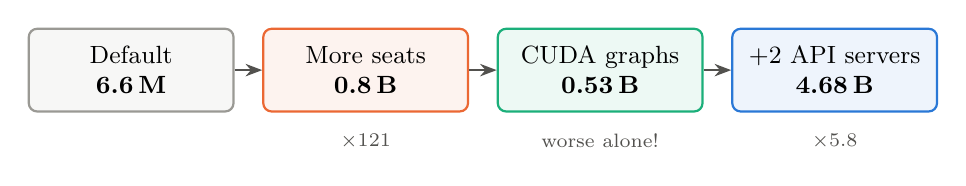
\begin{tikzpicture}[node distance=0.35cm]
  \node[blk=cgray,minimum width=2.6cm] (a) {Default\\\textbf{6.6\,M}};
  \node[blk=corange,minimum width=2.6cm,right=of a] (b) {More seats\\\textbf{0.8\,B}};
  \node[blk=caqua,minimum width=2.6cm,right=of b] (c) {CUDA graphs\\\textbf{0.53\,B}};
  \node[blk=cblue,minimum width=2.6cm,right=of c] (d) {+2 API servers\\\textbf{4.68\,B}};
  \draw[arr] (a)--(b); \draw[arr] (b)--(c); \draw[arr] (c)--(d);
  \node[below=0.15cm of b,font=\scriptsize\color{ink2}] {$\times$121};
  \node[below=0.15cm of c,font=\scriptsize\color{ink2}] {worse alone!};
  \node[below=0.15cm of d,font=\scriptsize\color{ink2}] {$\times$5.8};
\end{tikzpicture}
\end{center}

\vfill
{\color{accent}\rule{\linewidth}{0.6pt}}
\begin{center}\small\color{ink2}
Every number in this report comes from a result file in the repository.
Blue text is clickable: it opens the section, file or page it names.
\end{center}

\newpage
% =====================================================================
% CONTENTS + SUMMARY
% =====================================================================
\pdfbookmark[0]{Contents}{toc}
\begingroup\small
\setcounter{tocdepth}{1}
\tableofcontents
\endgroup

\begin{keybox}[The project in 30 seconds]
\begin{itemize}
  \item \textbf{Goal:} serve the vision-language model \texttt{Qwen3-VL-4B} with vLLM to many users at the same time, and get the highest score. The score rewards speed, many users and no errors, and it punishes every extra GPU.
  \item \textbf{What I did:} 21 load tests on one H100 GPU in about 80 minutes, for about \$5.50. Before each test I wrote down what I expected. After each test I checked which part of the system was the slowest.
  \item \textbf{What I found:} the GPU was \emph{not} the problem for most of the project. The slow parts were, in order: a limit of 32 requests at a time, the CPU work of launching GPU code, the single web-server process, and at the end my own load-testing tool.
  \item \textbf{Result:} score \textbf{4,680,469,940}, which is \textbf{705$\times$} the default setup on the same machine, with 0 errors.
\end{itemize}
\end{keybox}

% =====================================================================
\section{Introduction}
% =====================================================================
\subsection{What is this project?}
\textbf{InferTutor} is a pretend AI tutor. Students send questions. Some questions are short text, some are long reading passages, and some include a picture (a diagram or a chart). The model answers, and the answer \emph{streams}: the student sees the words appear one by one, like in ChatGPT.

My job was to run this service on real GPUs and make it as fast as possible for as many students as possible. I used:
\begin{itemize}
  \item \textbf{The model:} \texttt{Qwen3-VL-4B-Instruct}, a small model that reads text and images. Its weights are 8.9\,GB in bf16 (2 bytes per number), so it has about 4.4 billion parameters. On the 80\,GB GPU it used only 8.6\,GiB. vLLM gave 61\,GiB of the rest to the KV cache: room for 446,000 tokens at the same time (from the vLLM log).
  \item \textbf{The serving engine:} \href{https://github.com/vllm-project/vllm}{vLLM} 0.21.0. It loads the model on the GPU and offers an OpenAI-style web API.
  \item \textbf{The load tester:} a Python script from the course. It pretends to be many students. Each pretend student sends a question, reads the streamed answer, waits a short time (0.2--1.2\,s), and asks again.
\end{itemize}

\subsection{The four numbers that matter}
\begin{center}\small
\begin{tabularx}{\linewidth}{@{}l X l@{}}
\toprule
\textbf{Metric} & \textbf{What it means for a student} & \textbf{Want} \\
\midrule
TTFT p95 & \emph{Time To First Token}: how long until the first word appears. ``p95'' means 95\% of requests were faster than this. & low \\
ITL p95 & \emph{Inter-Token Latency}: the gap between two words. A big gap makes the text look jerky. & low \\
Throughput & How many streamed pieces (chunks) the server sends per second, for all users together. & high \\
Error rate & The share of requests that failed. & 0 \\
\bottomrule
\end{tabularx}
\end{center}

\subsection{The score}
\[
\text{Score} \;=\; \frac{\text{throughput} \times \text{users} \times (1-\text{error rate})}{\text{TTFT}_{p95} \times \text{ITL}_{p95} \times \text{number of GPUs}}
\]
\begin{note}[How to read the score]
\textbf{Users} is the number of pretend students \emph{I choose}. If the server stays fast, more users also means more throughput, so the score grows roughly with users$^2$. But if the server gets slow, the two latencies at the bottom grow and the score falls fast. So the real game is: \textbf{find the largest number of users the server can handle before it slows down}, then move that limit higher. Every extra GPU divides the score, so I used only \textbf{one}.
\end{note}

% =====================================================================
\section{Setup}
% =====================================================================
\subsection{Where everything runs}
The course examples use Modal. I rented one \textbf{H100 SXM} on \textbf{RunPod} for \$4.00 per hour and ran \emph{everything on that one machine}: the vLLM server and the load tester. The load tester talks to the server at \texttt{127.0.0.1}, so my home internet does not change the results.

\begin{center}
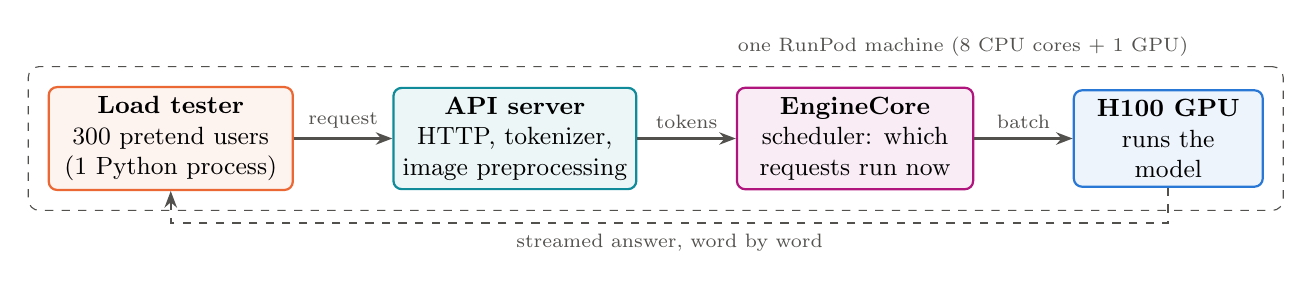
\begin{tikzpicture}[node distance=0.55cm and 0.5cm]
  \node[blk=corange,minimum width=3.1cm] (lt) {\textbf{Load tester}\\300 pretend users\\(1 Python process)};
  \node[blk=teal2,minimum width=3.0cm,right=1.25cm of lt] (api) {\textbf{API server}\\HTTP, tokenizer,\\image preprocessing};
  \node[blk=accent,minimum width=3.0cm,right=1.25cm of api] (eng) {\textbf{EngineCore}\\scheduler: which\\requests run now};
  \node[blk=cblue,minimum width=2.4cm,right=1.25cm of eng] (gpu) {\textbf{H100 GPU}\\runs the\\model};
  \draw[arr] (lt) -- node[above,font=\scriptsize]{request} (api);
  \draw[arr] (api) -- node[above,font=\scriptsize]{tokens} (eng);
  \draw[arr] (eng) -- node[above,font=\scriptsize]{batch} (gpu);
  \draw[arr,dashed] (gpu.south) -- ++(0,-0.45) -| node[pos=0.25,below,font=\scriptsize]{streamed answer, word by word} (lt.south);
  \node[draw=ink2,dashed,rounded corners=4pt,inner sep=7pt,fit=(lt)(api)(eng)(gpu),
        label={[font=\scriptsize\color{ink2}]above right:one RunPod machine (8 CPU cores + 1 GPU)}] {};
\end{tikzpicture}
\end{center}
Three of these boxes are \textbf{Python processes on the CPU}. This becomes very important later: one Python process can use at most \textbf{one CPU core}, even on an 8-core machine.

\subsection{Tools I built}
\begin{center}\small
\begin{tabularx}{\linewidth}{@{}l X@{}}
\toprule
\textbf{File} & \textbf{What it does} \\
\midrule
\file{tools/runpod_serve.sh} & Starts vLLM with the same flags as the course Modal app. Every knob is an environment variable. \\
\file{tools/runpod_matrix.sh} & Runs a list of experiments by name (for example \texttt{m-s256-300u}). Restarts vLLM only when a server knob changes, waits until it is healthy, and stops cleanly. \\
\file{tools/runpod_record.sh} & Records one run as a terminal video: live GPU stats on top, the load test below. \\
\file{tools/results_table.py} & Turns all result files into the score table in Section~\ref{sec:results}. \\
\file{tools/mock_vllm_server.py} & A fake server, so I could test all tools on my laptop (no GPU) before paying for one. \\
\bottomrule
\end{tabularx}
\end{center}

\begin{note}[A setup problem worth knowing]
The first start failed with \texttt{Can't load the configuration of 'Qwen/Qwen3-VL-4B-Instruct'}. The real cause was hidden: the RunPod template sets \texttt{HF\_HUB\_ENABLE\_HF\_TRANSFER=1}, but my new Python environment did not have the \texttt{hf\_transfer} package. Fix: \texttt{export HF\_HUB\_ENABLE\_HF\_TRANSFER=0}.
\end{note}

\subsection{How I worked}
\begin{center}
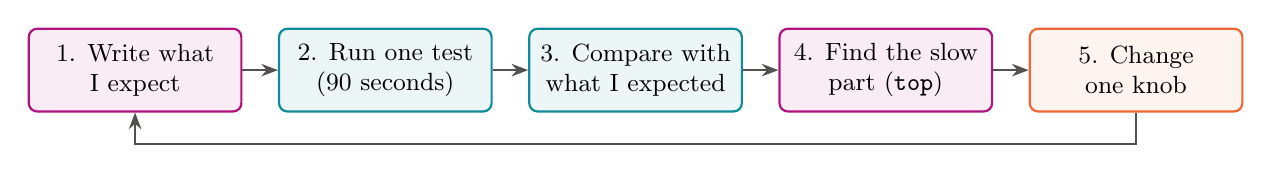
\begin{tikzpicture}[node distance=0.45cm]
  \node[blk=accent,minimum width=2.7cm] (h) {1. Write what\\I expect};
  \node[blk=teal2,minimum width=2.7cm,right=of h] (r) {2. Run one test\\(90 seconds)};
  \node[blk=teal2,minimum width=2.7cm,right=of r] (m) {3. Compare with\\what I expected};
  \node[blk=accent,minimum width=2.7cm,right=of m] (w) {4. Find the slow\\part (\texttt{top})};
  \node[blk=corange,minimum width=2.7cm,right=of w] (k) {5. Change\\one knob};
  \draw[arr] (h)--(r); \draw[arr] (r)--(m); \draw[arr] (m)--(w); \draw[arr] (w)--(k);
  \draw[arr] (k.south) -- ++(0,-0.4) -| (h.south);
\end{tikzpicture}
\end{center}
Each test: 90 seconds, 20 seconds of ramp-up, answers up to 96 tokens, mixed traffic (mostly text, some long passages, some images). The full log with every prediction is in \file{EXPERIMENTS.md}.

% =====================================================================
\section{Step 1 -- The waiting line (\texttt{max\_num\_seqs})}
% =====================================================================
\subsection{What I saw}
With the default setup, 50 users gave a score of 6.6\,M. I expected 100 users to give about twice the throughput. \textbf{It did not.} Throughput grew only 14\%, and TTFT went from 0.6\,s to 2.9\,s. At 150 users TTFT was 5.7\,s. Strangely, ITL stayed flat at about 20\,ms: the GPU was not slower, the requests were \emph{waiting}.

\begin{center}
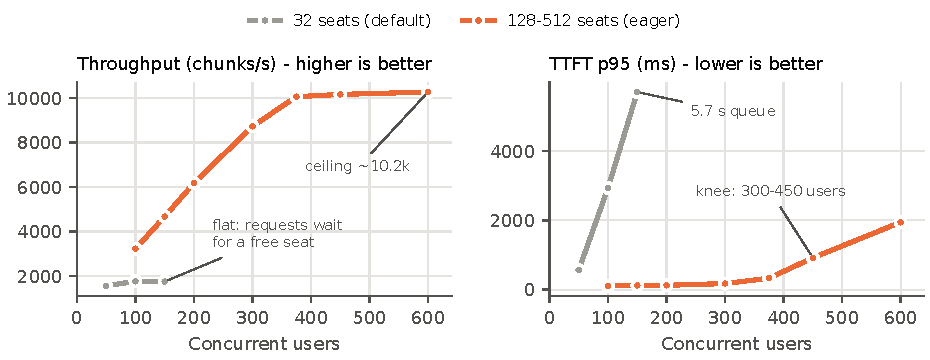
\includegraphics[width=\linewidth]{fig/fig_sweep.pdf}\\[-2pt]
{\small\color{ink2}Figure 1: Grey = default (32 seats). Orange = 128--512 seats. With 32 seats, throughput stops at about 1,770 chunks/s and the waiting time explodes.}
\end{center}

\subsection{Why it happens}
The knob \knob{max\_num\_seqs} is the number of requests vLLM works on at the same time. Think of it as \textbf{seats in a classroom}. The default is 32. With 100 students and 32 seats, the others wait at the door. Waiting time counts as TTFT.

\begin{center}
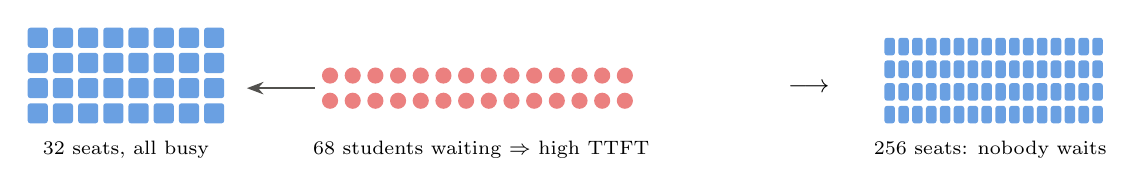
\begin{tikzpicture}[x=0.32cm,y=0.32cm]
  \foreach \i in {0,...,7} \foreach \j in {0,...,3}
    \fill[cblue!70,rounded corners=1pt] (\i,\j) rectangle ++(0.8,0.8);
  \node[font=\scriptsize,anchor=north] at (3.9,-0.3) {32 seats, all busy};
  \foreach \i in {0,...,13} \fill[cred!70] (12+\i*0.9,1.9) circle (0.32);
  \foreach \i in {0,...,13} \fill[cred!70] (12+\i*0.9,0.9) circle (0.32);
  \node[font=\scriptsize,anchor=north] at (18,-0.3) {68 students waiting $\Rightarrow$ high TTFT};
  \draw[arr] (11.4,1.4) -- (8.7,1.4);
  \node[font=\small\bfseries] at (31,1.4) {$\longrightarrow$};
  \foreach \i in {0,...,15} \foreach \j in {0,...,3}
    \fill[cblue!70,rounded corners=1pt] (34+\i*0.55,\j*0.9) rectangle ++(0.42,0.7);
  \node[font=\scriptsize,anchor=north] at (38.2,-0.3) {256 seats: nobody waits};
\end{tikzpicture}
\end{center}

More seats are almost free here. To make one new word for each request, the GPU must read all model weights once. Reading them once for 32 requests or for 256 requests costs nearly the same time. This is what ``decoding is memory-bound'' means.

\subsection{Result}
\begin{center}\small
\begin{tabular}{@{}lrrrrr@{}}
\toprule
\textbf{Seats, users} & \textbf{TTFT p95} & \textbf{ITL p95} & \textbf{Throughput} & \textbf{Score} & \textbf{vs default} \\
\midrule
32, 100 users & 2,936 ms & 19.5 ms & 1,773 & 3.1\,M & 1$\times$ \\
64, 100 users & 507 ms & 21.1 ms & 3,139 & 29\,M & 9.5$\times$ \\
128, 100 users & \textbf{106 ms} & 25.4 ms & 3,232 & \textbf{121\,M} & \textbf{39$\times$} \\
256, 300 users & 175 ms & 24.9 ms & 8,727 & 600\,M & -- \\
\bottomrule
\end{tabular}
\end{center}
With more seats I could raise the number of users to 300 before TTFT started to grow (the \emph{knee} is between 300 and 450 users, Figure~1).

% =====================================================================
\section{Step 2 -- The CPU, not the GPU (CUDA graphs)}
% =====================================================================
\subsection{What I saw}
At 300 users the RunPod dashboard showed the GPU busy only about \textbf{40\%} of the time. ITL stayed near 25\,ms whether 100 or 300 users were active. If the GPU were the limit, ITL would grow with more users. So I opened \texttt{top} during a test (Figure~2, left): the \texttt{VLLM::EngineCore} process was at \textbf{100\% CPU}, which means one full core.

\begin{center}
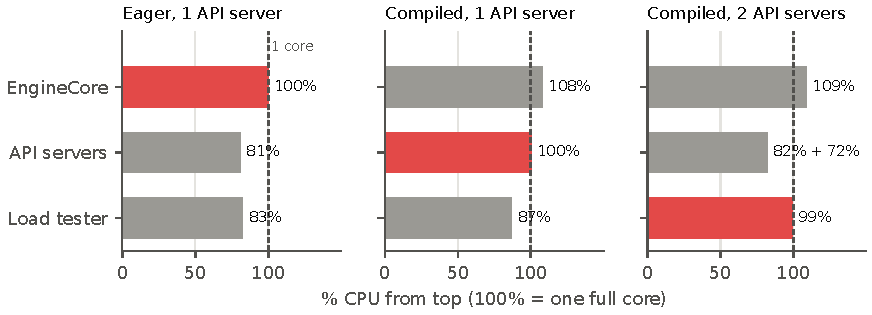
\includegraphics[width=\linewidth]{fig/fig_cpu.pdf}\\[-2pt]
{\small\color{ink2}Figure 2: CPU use of the three Python processes from \texttt{top}, during the load test. Red = the process that is full (the bottleneck). The bottleneck moves every time I fix one.}
\end{center}

\subsection{Why it happens}
In the default \emph{eager} mode, the CPU sends every small GPU task (a ``kernel'') one by one. A 4B model is small for an H100, so each GPU task is short and the GPU waits for the CPU between tasks. \textbf{CUDA graphs} record all the tasks of one step once, and then replay them with one command.

\begin{center}
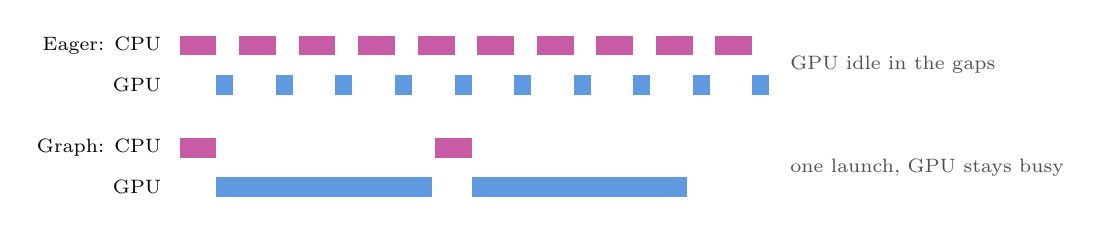
\begin{tikzpicture}[x=0.36cm,y=0.5cm]
  \node[anchor=east,font=\scriptsize] at (-0.3,1) {Eager: CPU};
  \node[anchor=east,font=\scriptsize] at (-0.3,0) {GPU};
  \foreach \i in {0,...,9} {
    \fill[accent!70] (\i*2.1,0.75) rectangle ++(1.3,0.5);
    \fill[cblue!75] (\i*2.1+1.3,-0.25) rectangle ++(0.6,0.5);
  }
  \node[anchor=west,font=\scriptsize\color{ink2}] at (21.2,0.5) {GPU idle in the gaps};
  \node[anchor=east,font=\scriptsize] at (-0.3,-1.6) {Graph: CPU};
  \node[anchor=east,font=\scriptsize] at (-0.3,-2.6) {GPU};
  \fill[accent!70] (0,-1.85) rectangle ++(1.3,0.5);
  \fill[cblue!75] (1.3,-2.85) rectangle ++(7.6,0.5);
  \fill[accent!70] (9.0,-1.85) rectangle ++(1.3,0.5);
  \fill[cblue!75] (10.3,-2.85) rectangle ++(7.6,0.5);
  \node[anchor=west,font=\scriptsize\color{ink2}] at (21.2,-2.1) {one launch, GPU stays busy};
\end{tikzpicture}
\end{center}

\subsection{Result -- a surprise}
Compiled mode (\knob{--no-enforce-eager}) cut ITL from about 21--25\,ms to \textbf{8.5\,ms}, three times better, and throughput rose 43\%. \textbf{But the score went down} (600\,M $\rightarrow$ 533\,M), because TTFT jumped to \textbf{832\,ms} (Figure~3, middle bars).

% =====================================================================
\section{Step 3 -- The web server (\texttt{--api-server-count})}
% =====================================================================
\subsection{A wrong guess first}
Faster words mean each student finishes sooner and asks again sooner: requests per second rose from about 86 to 145. My first guess was that new prompts were waiting for GPU time. The knob for this is the prefill budget,\\ \knob{max\_num\_batched\_tokens}. I doubled it from 4096 to 8192. \textbf{TTFT got worse} (962\,ms), so the guess was wrong. I kept this result in the log.

\subsection{What \texttt{top} showed}
In compiled mode the EngineCore had room again, but the \textbf{API server was at 100\% CPU} (Figure~2, middle). The API server does a lot of work before a request reaches the GPU: it reads HTTP, turns text into tokens, prepares the image, and sends about 12,000 chunks per second back to 300 users. All of this happened in \emph{one} Python process. Every new request waited for it, and that waiting is part of TTFT.

\subsection{The fix and the result}
vLLM 0.21.0 can start several API server processes with \knob{--api-server-count}. I checked the vLLM source code for this version first; the default is 1. With \textbf{2 API servers}, they ran at 82\% and 72\% CPU (not full), and:

\begin{center}
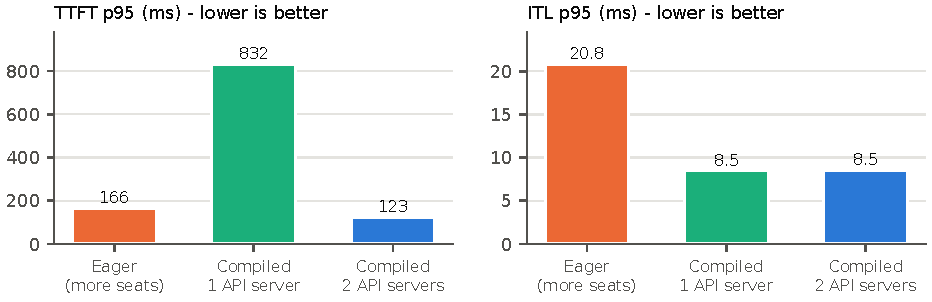
\includegraphics[width=\linewidth]{fig/fig_tradeoff.pdf}\\[-2pt]
{\small\color{ink2}Figure 3: Compiled mode alone made words faster (right) but the first word slower (left). Adding a second API server fixed the first word and kept the fast words.}
\end{center}

\begin{keybox}[Why this matters]
CUDA graphs and 2 API servers only help \textbf{together}. Each one alone moved the bottleneck to a different place. Together they gave \textbf{TTFT 123\,ms, ITL 8.5\,ms and 16,375 chunks/s}, and the GPU was busy \textbf{87\%} of the time (536\,W, from \texttt{nvidia-smi} during the final run).
\end{keybox}

% =====================================================================
\section{Knobs that did not matter -- and the noise}
% =====================================================================
I also tested four common knobs at 300 users: prefix caching off, chunked prefill off, and batch tokens 2048 and 8192. All results were between 600\,M and 767\,M. Then I ran the \emph{same} baseline setup again, 30 minutes later: it scored \textbf{802\,M}, which is 34\% higher than the first time (600\,M).

\begin{center}
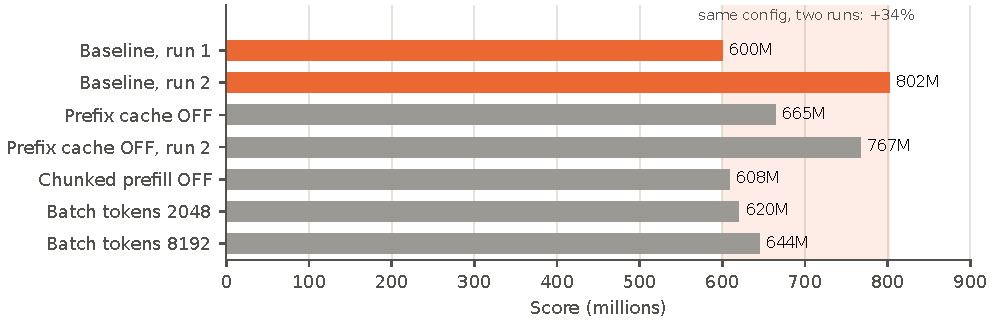
\includegraphics[width=0.92\linewidth]{fig/fig_noise.pdf}\\[-2pt]
{\small\color{ink2}Figure 4: The shaded band is the difference between two runs of the same setup. Every knob result falls inside or near it.}
\end{center}

So these four knobs had \textbf{no effect I can measure} at this noise level. My explanation (not proven): the machine is shared with other customers (load average 50--70), and my bottleneck was a CPU process, so other customers' work changes my speed. The score multiplies two p95 values, so small changes become bigger. Only changes much bigger than 30\% are real here: more seats (39$\times$) and the final setup (5.8$\times$) are. The final setup was also run twice: 4.41\,B and 4.68\,B, only 6\% apart.

% =====================================================================
\newpage
\section{All results}\label{sec:results}
% =====================================================================
\begin{center}
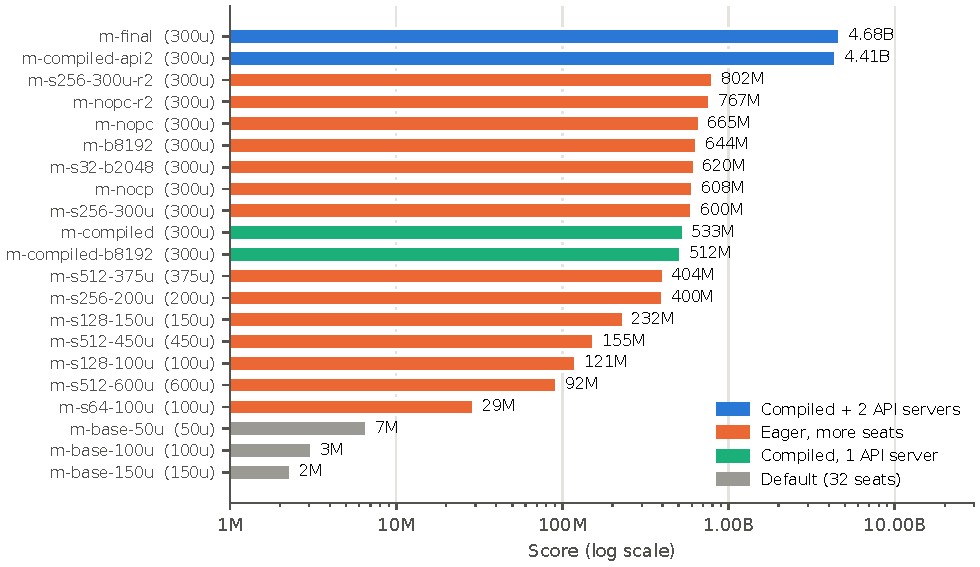
\includegraphics[width=0.94\linewidth]{fig/fig_scores.pdf}\\[-2pt]
{\small\color{ink2}Figure 5: All 21 runs, sorted by score (log scale). Colour = setup family.}
\end{center}

\begin{center}\scriptsize
\setlength{\tabcolsep}{3.6pt}
\begin{tabular}{@{}rlllrrrrr@{}}
\toprule
\# & \textbf{Run} & \textbf{Seats / batch tokens} & \textbf{Mode} & \textbf{Users} & \textbf{TTFT p95} & \textbf{ITL p95} & \textbf{Chunks/s} & \textbf{Score} \\
\midrule
1 & \texttt{m-final} & 256 / 4096, 2 API servers & compiled & 300 & 123 ms & 8.5 ms & 16,375 & \textbf{4,680,469,940} \\
2 & \texttt{m-compiled-api2} & 256 / 4096, 2 API servers & compiled & 300 & 127 ms & 8.7 ms & 16,182 & 4,414,646,436 \\
3 & \texttt{m-s256-300u-r2} & 256 / 4096 & eager & 300 & 166 ms & 20.8 ms & 9,249 & 802,031,590 \\
4 & \texttt{m-nopc-r2} & 256 / 4096, no prefix cache & eager & 300 & 164 ms & 21.9 ms & 9,148 & 766,715,333 \\
5 & \texttt{m-nopc} & 256 / 4096, no prefix cache & eager & 300 & 168 ms & 23.7 ms & 8,794 & 664,754,094 \\
6 & \texttt{m-b8192} & 256 / 8192 & eager & 300 & 182 ms & 23.2 ms & 9,075 & 644,390,229 \\
7 & \texttt{m-s32-b2048} & 256 / 2048 & eager & 300 & 176 ms & 24.1 ms & 8,797 & 620,163,376 \\
8 & \texttt{m-nocp} & 256 / 4096, no chunked prefill & eager & 300 & 159 ms & 25.7 ms & 8,309 & 608,271,121 \\
9 & \texttt{m-s256-300u} & 256 / 4096 & eager & 300 & 175 ms & 24.9 ms & 8,727 & 600,035,679 \\
10 & \texttt{m-compiled} & 256 / 4096 & compiled & 300 & 832 ms & 8.5 ms & 12,478 & 532,509,459 \\
11 & \texttt{m-compiled-b8192} & 256 / 8192 & compiled & 300 & 962 ms & 7.7 ms & 12,721 & 512,379,078 \\
12 & \texttt{m-s512-375u} & 512 / 4096 & eager & 375 & 330 ms & 28.3 ms & 10,054 & 404,192,017 \\
13 & \texttt{m-s256-200u} & 256 / 4096 & eager & 200 & 125 ms & 24.7 ms & 6,177 & 400,255,026 \\
14 & \texttt{m-s128-150u} & 128 / 4096 & eager & 150 & 123 ms & 24.5 ms & 4,672 & 232,235,517 \\
15 & \texttt{m-s512-450u} & 512 / 4096 & eager & 450 & 918 ms & 32.2 ms & 10,160 & 154,781,376 \\
16 & \texttt{m-s128-100u} & 128 / 4096 & eager & 100 & 106 ms & 25.4 ms & 3,232 & 120,565,085 \\
17 & \texttt{m-s512-600u} & 512 / 4096 & eager & 600 & 1,946 ms & 34.3 ms & 10,266 & 92,321,708 \\
18 & \texttt{m-s64-100u} & 64 / 4096 & eager & 100 & 507 ms & 21.1 ms & 3,139 & 29,361,553 \\
19 & \texttt{m-base-50u} & 32 / 4096 (default) & eager & 50 & 565 ms & 20.8 ms & 1,559 & 6,634,027 \\
20 & \texttt{m-base-100u} & 32 / 4096 (default) & eager & 100 & 2,936 ms & 19.5 ms & 1,773 & 3,095,106 \\
21 & \texttt{m-base-150u} & 32 / 4096 (default) & eager & 150 & 5,706 ms & 19.8 ms & 1,757 & 2,327,456 \\
\bottomrule
\end{tabular}\\[2pt]
{\color{ink2}All runs: 1 GPU, 0 errors, mixed traffic, 90\,s. Raw files: \file{starter_code/results_infertutor}.}
\end{center}

\subsection{The final setup}
\begin{lstlisting}
# server (from submission/final_command.sh)
vllm serve Qwen/Qwen3-VL-4B-Instruct --max-num-seqs 256 --max-num-batched-tokens 4096 \
  --no-enforce-eager --api-server-count 2 --enable-prefix-caching --enable-chunked-prefill \
  --max-model-len 8192 --gpu-memory-utilization 0.90 --dtype bfloat16
# load test: 300 users, mixed traffic, 90 s
python run_infertutor_experiment.py --url http://127.0.0.1:8000 --label m-final \
  --mode mixed --users 300 --max-seqs 256 --no-fast-boot
\end{lstlisting}
Exact commands: \file{submission/final_command.sh}. Result file: \file{submission/final_result.json}.

% =====================================================================
\newpage
\section{Lessons, limits and next steps}
% =====================================================================
\subsection{The bottleneck moved four times}
\begin{center}
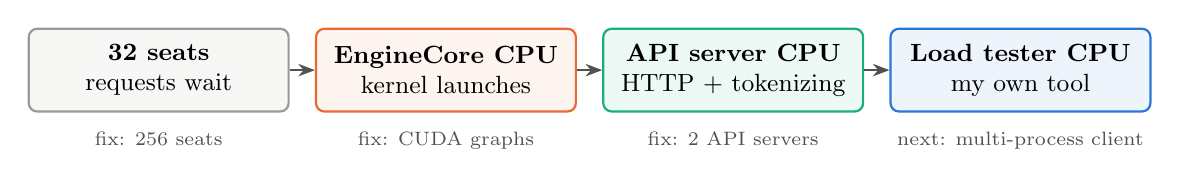
\begin{tikzpicture}[node distance=0.32cm]
  \node[blk=cgray,minimum width=3.3cm] (a) {\textbf{32 seats}\\requests wait};
  \node[blk=corange,minimum width=3.3cm,right=of a] (b) {\textbf{EngineCore CPU}\\kernel launches};
  \node[blk=caqua,minimum width=3.3cm,right=of b] (c) {\textbf{API server CPU}\\HTTP + tokenizing};
  \node[blk=cblue,minimum width=3.3cm,right=of c] (d) {\textbf{Load tester CPU}\\my own tool};
  \draw[arr] (a)--(b); \draw[arr] (b)--(c); \draw[arr] (c)--(d);
  \node[below=0.12cm of a,font=\scriptsize\color{ink2}] {fix: 256 seats};
  \node[below=0.12cm of b,font=\scriptsize\color{ink2}] {fix: CUDA graphs};
  \node[below=0.12cm of c,font=\scriptsize\color{ink2}] {fix: 2 API servers};
  \node[below=0.12cm of d,font=\scriptsize\color{ink2}] {next: multi-process client};
\end{tikzpicture}
\end{center}

\subsection{What I learned}
\begin{enumerate}
  \item \textbf{Measure before you tune.} A 14\% throughput gain for 2$\times$ users told me requests were waiting, not computing.
  \item \textbf{Low GPU use is a clue, not a goal.} 40\% GPU use meant the CPU could not feed the GPU fast enough.
  \item \textbf{Fixing one bottleneck shows the next one.} CUDA graphs alone made the score worse, because they moved the problem to the API server.
  \item \textbf{Repeat runs.} One repeated run showed 34\% noise and stopped me from making wrong claims about prefix caching.
  \item \textbf{Keep wrong guesses.} The bigger-prefill-budget guess was wrong, and \texttt{top} found the real cause.
\end{enumerate}

\subsection{Honest limits}
\begin{itemize}
  \item \textbf{The final run was limited by my load tester.} It used 99\% of one CPU core at 16k chunks/s. The server can probably do more than I measured, and I did not test more than 300 users with the final setup.
  \item \textbf{Not comparable to the course reference} (about 3.3\,M on 2 GPUs). That test ran its load tester on a laptop over the internet, so its TTFT includes network time. Mine does not.
  \item Most runs were done once. Only the baseline, prefix-cache-off and final setups were repeated.
  \item The result file cannot store \texttt{--api-server-count}; the run name and the vLLM log record it.
\end{itemize}

\subsection{Next steps}
A load tester with several processes, then a user sweep (300 $\rightarrow$ 600) and 3--4 API servers on the final setup; three repeats for each knob; the text-only track; and FP8 for the KV cache, checked against answer quality first.

\section{Glossary and how to reproduce}
\subsection{Words used in this report}
\begin{center}\small
\begin{tabularx}{\linewidth}{@{}l X@{}}
\toprule
\textbf{Word} & \textbf{Simple meaning} \\
\midrule
Token & A small piece of text, about 3/4 of a word. The model reads and writes tokens. \\
Prefill & The first phase: the model reads the whole question (and image) at once. It decides TTFT. \\
Decode & The second phase: the model writes the answer, one token per step. It decides ITL. \\
Batching & The GPU works on many requests in the same step. vLLM adds a new request as soon as a seat is free (\emph{continuous batching}). \\
KV cache & GPU memory where the model keeps what it has already read, so it does not read it again. \\
Prefix caching & If many prompts start with the same text (like a system prompt), reuse that work. \\
Chunked prefill & Cut a long prompt into pieces, so it does not stop other users' words for too long. \\
Eager mode & The CPU sends every GPU task one by one. Simple, but slow for small models. \\
CUDA graph & A recording of all GPU tasks of one step, replayed with one command (\emph{compiled mode}). \\
p95 & Sort all requests from fast to slow; p95 is the value that 95\% of requests are faster than. \\
Bottleneck & The slowest part of a system. Making other parts faster does not help until it is fixed. \\
\bottomrule
\end{tabularx}
\end{center}

\subsection{Timeline of the session (19 October 2026, IST)}
\begin{center}\small
\renewcommand{\arraystretch}{1.12}
\begin{tabularx}{\linewidth}{@{}l X r@{}}
\toprule
\textbf{Time} & \textbf{What happened} & \textbf{Best score} \\
\midrule
16:58 & Rented 1$\times$ H100 SXM on RunPod (\$4.00/hour). Installed vLLM 0.21.0. & -- \\
17:10 & First start failed (\texttt{hf\_transfer}, Section 2). Fixed; model downloaded in 24\,s. & -- \\
17:15 & First test, default setup, 50 users. 0 errors. & 6.6\,M \\
17:19 & 100 and 150 users: requests wait in a queue (Step 1). & 6.6\,M \\
17:33 & More seats (64 $\rightarrow$ 256), up to 300 users. & 600\,M \\
17:42 & 375--600 users: found the knee and a ceiling at $\sim$10.2k chunks/s. & 600\,M \\
17:45 & CUDA graphs: words 3$\times$ faster, first word slower (Step 2). \texttt{top}: EngineCore at 100\%. & 600\,M \\
17:54 & Four knob tests (prefix cache, chunked prefill, batch tokens). & 665\,M \\
18:01 & Wrong guess: bigger prefill budget. \texttt{top}: API server at 100\% (Step 3). & 665\,M \\
18:05 & Repeat runs: the same setup varies by 34\%. & 802\,M \\
18:08 & CUDA graphs + 2 API servers. & \textbf{4.41\,B} \\
18:14 & Final run, recorded as a video. & \textbf{4.68\,B} \\
18:20 & Downloaded all results, stopped and deleted the machine. Total about 82 minutes, about \$5.50. & -- \\
\bottomrule
\end{tabularx}
\end{center}

\subsection{Run it yourself}
\noindent\begin{minipage}{\linewidth}
\begin{lstlisting}
git clone https://github.com/himanshu1573/qwen-vl-inference-arena.git && cd qwen-vl-inference-arena
uv venv --python 3.12 && source .venv/bin/activate
uv pip install "vllm==0.21.0" "qwen-vl-utils==0.0.14" -r starter_code/requirements.txt
export HF_HUB_ENABLE_HF_TRANSFER=0          # needed on the RunPod PyTorch template
tools/runpod_matrix.sh m-base-50u m-s256-300u  # any experiment from EXPERIMENTS.md
submission/final_command.sh                    # the final run
\end{lstlisting}
\end{minipage}
More detail: \file{README.md} (setup), \file{EXPERIMENTS.md} (every run with its prediction), \file{REPORT.md} (one-page version).

\begin{tcolorbox}[colback=soft,colframe=accent,arc=3pt,boxrule=0.6pt,title={\small\bfseries Skills shown in this project}]
\small
LLM serving with vLLM $\cdot$ GPU performance tuning (batching, CUDA graphs, API scaling) $\cdot$ load testing and p95 latency analysis $\cdot$ finding bottlenecks with \texttt{top} and \texttt{nvidia-smi} $\cdot$ reading framework source code $\cdot$ experiment design with written hypotheses $\cdot$ Bash and Python tooling $\cdot$ cloud GPUs on a \$13 budget. \hfill \href{\repo}{\textbf{View the code on GitHub}}
\end{tcolorbox}

\end{document}
